\documentclass[12pt]{article}
%\usepackage[utf8]{inputenc} %Paquete para poder poner acentos desde el teclado. No lo necesitamos con XeLaTeX si usamos \usepackage{fontspec}
\usepackage{fontspec} %Paquete de fuentes avanzado (sólo XeLaTeX)

%%%%%%%%%%%%%%%%%%%%%%%%%%%%%%%%%%%%%%%%%%%%%%%%%%%%%%%%%%%%%%%%%%%%%%%%%%%%%
%% FUENTES %%%%%%%%%%%%%%%%%%%%%%%%%%%%%%%%%%%%%%%%%%%%%%%%%%%%%%%%%%%%%%%%%%%%%%%%%%%%%%%


%\usepackage{mathptmx} %Times New Roman
%\setmainfont{Arial} %Arial. Sólo XeLaTeX

%%%%%%%%%%%%%%%%%%%%%%%%%%%%%%%%%%%%%%%%%%%%%%%%%%%%%%%%%%%%%%%%%%%%%%%%%%%%%%%


%%%%%%%%%%%%%%%%%%%%%%%%%%%%%%%%%%%%%%%%%%%%%%%%%%%%%%%%%%%%%%%%%%%%%%%%%%%%%%% PAQUETES BÁSICOS %%%%%%%%%%%%%%%%%%%%%%%%%%%%%%%%%%%%%%%%%%%%%%%%%%%%%%%%%%%%%%%%%%%%%%%%%%%%%%%


%\usepackage[spanish]{babel} %Paquete para que el documento esté en español. Quitar "spanish" para tener el índice en inglés
\usepackage{polyglossia} %Paquete igual que "babel" pero para XeLaTex. Permite eliminar la primera sangría con otro comando (ver sección "Distancias".
\setmainlanguage{spanish} %Lenguaje del texto cuando usas polyglossia
\usepackage{eurosym} %Paquete para poder meter el símbolo €
\usepackage{amsmath} %Paquete básico para matemáticas
\usepackage{graphicx} %Paquete para incluir imágenes
\usepackage{hyperref} %Paquete para poder poner hipervínculos
\hypersetup{
    colorlinks=true,
    linkcolor=blue,
    filecolor=magenta,      
    urlcolor=cyan,
    pdftitle={Primera entrega - Manuel de la Llave},
    bookmarksopen=true,
    citecolor=RawSienna,
} %Opciones de los hipervínculos y cross references.
\usepackage{cleveref} %Paquete para mejorar las referencias cruzadas.
\usepackage{enumerate} %Paquete para cambiar los números en las listas numeradas
\usepackage{enumitem} %Paquete para modificar las listas
\usepackage{multicol} %Paquete para crear multicolumnas
\usepackage{parskip} %Paquete para que se espacien los párrafos
\usepackage{array} %Paquete para dar mejor formato a las tablas
\usepackage{rotating} %Paquete para poder rotar tablas
\usepackage{float} %Paquete para colocar mejor las imágenes
\usepackage{csquotes} %Paquete para mejorar la edición de citas
\usepackage[nottoc]{tocbibind} %Paquete para añadir la bibliografía y otros elementos a la table of contents. nottoc = Not Table of Contents. Se puede poner notbib, notindex, etc.
\usepackage{epigraph} %Paquete para poder poner epígrafes
\usepackage{dirtytalk} %Paquete para poner citas usando \say{}
\usepackage[normalem]{ulem} %Paquete para subrayar (underline); normalem se usa para que no sutituya las itálicas por subrayados para enfatizar.
\useunder{\uline}{\ul}{} %Para personalizar el subrayado.
\usepackage{lscape} %Paquete para poder rotar páginas.
\usepackage{geometry}%Paquete para modificar los márgenes de manera más avanzada.
\usepackage{cancel} %Paquete para cancelar (tachar) elementos 
\usepackage[dvipsnames]{xcolor} %Paquete para aumentar las opciones de cambiar colores.
\usepackage{unicode-math} %Paquete para implementar unicode maths. Por ejemplo, para la epsilon mayúscula, \Eulerconst, necesita este paquete.
\usepackage[stable]{footmisc} %Paquete para dar más opciones en los footnote. Stable para poder poner footnotes en las cabeceras de las secciones y subsecciones.
\usepackage{optidef} %Paquete para problemas de optimización con \begin{mini/maxi}
\usepackage{pdfpages} %Paquete para incluir páginas de PDF en el documento.
\usepackage{bibentry} %Paquete para no incluir la sección bibliografía usando \nobibliography{name.bib} pero seguir citando
\usepackage{verbatim} %Paquete para hacer más cosas con verbatim


%%%%%%%%%%%%%%%%%%%%%%%%%%%%%%%%%%%%%%%%%%%%%%%%%%%%%%%%%%%%%%%%%%%%%%%%%%%%%%%


%%%%%%%%%%%%%%%%%%%%%%%%%%%%%%%%%%%%%%%%%%%%%%%%%%%%%%%%%%%%%%%%%%%%%%%%%%%%%%% BIBLIOGRAFÍA %%%%%%%%%%%%%%%%%%%%%%%%%%%%%%%%%%%%%%%%%%%%%%%%%%%%%%%%%%%%%%%%%%%%%%%%%%%%%%%


\usepackage{natbib}
\bibliographystyle{agsm} %Formato Harvard
\setcitestyle{authoryear-ibid,open={(},close={)}} 

%%%%%%%%%%%%%%%%%%%%%%%%%%%%%%%%%%%%%%%%%%%%%%%%%%%%%%%%%%%%%%%%%%%%%%%%%%%%%%%


%%%%%%%%%%%%%%%%%%%%%%%%%%%%%%%%%%%%%%%%%%%%%%%%%%%%%%%%%%%%%%%%%%%%%%%%%%%%%%% CAMBIOS DISTANCIAS %%%%%%%%%%%%%%%%%%%%%%%%%%%%%%%%%%%%%%%%%%%%%%%%%%%%%%%%%%%%%%%%%%%%%%%%%%%%%%%

\geometry{
 a4paper,
 left=30mm,
 right=30mm,
 top=25mm,
 bottom=25mm,
 heightrounded, % Ensures the height is adjusted so that an integer number of lines are accommodated in the text block.
 } 
\setlength{\parskip}{0cm} %Distancia entre párrafos. El plus y minus es el margen que le das a LaTeX para modificar el espaciado si lo considera necesario
\setlength{\parindent}{0.4cm} %Sangría
\renewcommand{\baselinestretch}{1} %Espaciado entre líneas. Por defecto es 1.
\PolyglossiaSetup{spanish}{indentfirst=false}

%%%%%%%%%%%%%%%%%%%%%%%%%%%%%%%%%%%%%%%%%%%%%%%%%%%%%%%%%%%%%%%%%%%%%%%%%%%%%%%


%%%%%%%%%%%%%%%%%%%%%%%%%%%%%%%%%%%%%%%%%%%%%%%%%%%%%%%%%%%%%%%%%%%%%%%%%%%%%%% NUEVOS COMANDOS %%%%%%%%%%%%%%%%%%%%%%%%%%%%%%%%%%%%%%%%%%%%%%%%%%%%%%%%%%%%%%%%%%%%%%%%%%%%%%%

% Keywords command
\providecommand{\keywords}[1]
{
  \small	
  \textbf{\textit{Palabras clave:}} #1
}

\providecommand{\ie}
{
\textit{i.e.}
}

%Fuente dentro del caption en las figuras
\newcommand*{\captionsource}[2]{%
  \caption[{#1}]{%
    #1%
    \\\hspace{\linewidth}%
    \textbf{Fuente:} #2%
  }%
}


\addto{\captionsspanish}{\renewcommand{\refname}{Bibliografía}} %Para cambiar el nombre de la bibliogradía usando el paquete "babel". "refname" para "article", "bibname" para "book" o "report". Si no usas babel, con \renewcommand{\bibname}{Bibliografía} es suficiente

%%%%%%%%%%%%%%%%%%%%%%%%%%%%%%%%%%%%%%%%%%%%%%%%%%%%%%%%%%%%%%%%%%%%%%%%%%%%%%%



%%%%%%%%%%%%%%%%%%%%%%%%%%%%%%%%%%%%%%%%%%%%%%%%%%%%%%%%%%%%%%%%%%%%%%%%%%%%%%% OTROS %%%%%%%%%%%%%%%%%%%%%%%%%%%%%%%%%%%%%%%%%%%%%%%%%%%%%%%%%%%%%%%%%%%%%%%%%%%%%%%

\numberwithin{equation}{section} %Para enumerar las ecuaciones por sección.
\setcounter{secnumdepth}{0} %Para que párrafos y subpárrafos cuenten como secciones en el índice, nivel de profundidad 4 y 5 respectivamente. 0 Para que no se numere el índice.
\setcounter{tocdepth}{3} %Nivel de profundidad de la Table Of Contents



%%%%%%%%%%%%%%%%%%%%%%%%%%%%%%%%%%%%%%%%%%%%%%%%%%%%%%%%%%%%%%%%%%%%%%%%%%%%%%%

\begin{document}

\renewcommand*{\thefootnote}{\fnsymbol{footnote}} %Comando para poner símbolos sobre el nombre del autor



\begin{titlepage} %

	\newcommand{\HRule}{\rule{\linewidth}{0.5mm}} % Defines a new command for horizontal lines, change thickness here
	
	\center % Centre everything on the page
	
	%------------------------------------------------
	%	Headings
	%------------------------------------------------
	
	%\includegraphics[width=\textwidth]{Images/spain.jpg}\\[1cm]
	
	%\textsc{\LARGE Universidad de Valencia}\\[1.5cm] % Main heading such as the name of your university/college
	
	%\textsc{\Large Facultad de Economía}\\[0.5cm] % Major heading such as course name
	
	%\textsc{\large Minor Heading}\\[0.5cm] % Minor heading such as course title
	
	%------------------------------------------------
	%	Title
	%------------------------------------------------
	
	\HRule\\[0.4cm]
	
	{\huge\bfseries Primera práctica de evaluación
	}\\[0.4cm] % Title of your document
	
	\HRule\\[1.5cm]
	
	\vfill
	%------------------------------------------------
	%	Author(s)
	%------------------------------------------------
	%\begin{multicols}{2}
	%\begin{minipage}{0.4\textwidth}
		%\begin{flushleft}
			\large
			\textit{Autor}\\
			Manuel \textsc{de la Llave}\footnote{llave@alumni.uv.es}
			\\
			%\columnbreak
		%\end{flushleft}
	%\end{minipage}
	~
	%\begin{minipage}{0.4\textwidth}
	%	\begin{flushright}
			%\large
			%\textit{Profesor}\\
			%Vicente \textsc{Esteve} % Supervisor's name
	%	\end{flushright}
	%\end{minipage}
	%\end{multicols}
	% If you don't want a supervisor, uncomment the two lines below and comment the code above
	%{\large\textit{Author}}\\
	%John \textsc{Smith} % Your name
	
	%------------------------------------------------
	%	Date
	%------------------------------------------------
	
	\vfill\vfill\vfill % Position the date 3/4 down the remaining page
	
	{\large 9 de Febrero de 2020} % Date, change the \today to a set date if you want to be precise
	
	%------------------------------------------------
	%	Logo
	%------------------------------------------------
	
	%\vfill\vfill
	%\includegraphics[width=0.2\textwidth]{logouv.png}\\[1cm] % Include a department/university logo - this will require the graphicx package
	 
	%----------------------------------------------------------------------------------------
	
	\vfill % Push the date up 1/4 of the remaining page
	
\end{titlepage}


\clearpage
\tableofcontents
\clearpage


\setcounter{footnote}{0} %Para que la página del título no cuente como página a la hora de numerar.
\renewcommand*{\thefootnote}{\arabic{footnote}} %Para que las notas al pie vuelvan a ser 1, 2, 3, etc. y no el símbolo como en el autor.

Considera el modelo de tres factores:

\begin{equation}\label{maineq}
    HiTec − R_f = \beta_1 + \beta_2(R_m-R_f) + \beta_3smb + \beta_4hml + u
\end{equation}


\section{Ejercicio 1} Estima la regresión lineal y muestra los resultados. Interpreta cada uno de los coeficientes del modelo.

\begin{table}[!h]
\centering
\begin{tabular}{lrrrr}
\multicolumn{3}{l}{Dependent Variable: HITEC-RF}&\multicolumn{1}{c}{}&\multicolumn{1}{c}{}\\
\multicolumn{2}{l}{Method: Least Squares}&\multicolumn{1}{c}{}&\multicolumn{1}{c}{}&\multicolumn{1}{c}{}\\
\multicolumn{2}{l}{Date: 09/02/20   Time: 15:17}&\multicolumn{1}{c}{}&\multicolumn{1}{c}{}&\multicolumn{1}{c}{}\\
\multicolumn{2}{l}{Sample: 1926M07 2015M12}&\multicolumn{1}{c}{}&\multicolumn{1}{c}{}&\multicolumn{1}{c}{}\\
\multicolumn{3}{l}{Included observations: 1074}&\multicolumn{1}{c}{}&\multicolumn{1}{c}{}\\
[4.5pt] \hline \\ [-4.5pt]
\multicolumn{1}{c}{Variable}&\multicolumn{1}{r}{Coefficient}&\multicolumn{1}{r}{Std. Error}&\multicolumn{1}{r}{t-Statistic}&\multicolumn{1}{r}{Prob.}\\
[4.5pt] \hline \\ [-4.5pt]
\multicolumn{1}{c}{C}&\multicolumn{1}{r}{$0.138453$}&\multicolumn{1}{r}{$0.063893$}&\multicolumn{1}{r}{$2.166956$}&\multicolumn{1}{r}{$0.0305$}\\
\multicolumn{1}{c}{RMRF}&\multicolumn{1}{r}{$0.986237$}&\multicolumn{1}{r}{$0.012658$}&\multicolumn{1}{r}{$77.91150$}&\multicolumn{1}{r}{$0.0000$}\\
\multicolumn{1}{c}{SMB}&\multicolumn{1}{r}{$0.041632$}&\multicolumn{1}{r}{$0.020747$}&\multicolumn{1}{r}{$2.006691$}&\multicolumn{1}{r}{$0.0450$}\\
\multicolumn{1}{c}{HML}&\multicolumn{1}{r}{$-0.319994$}&\multicolumn{1}{r}{$0.018407$}&\multicolumn{1}{r}{$-17.38404$}&\multicolumn{1}{r}{$0.0000$}\\
[4.5pt] \hline \\ [-4.5pt]
\multicolumn{1}{l}{R-squared}&\multicolumn{1}{r}{$0.864345$}&\multicolumn{2}{l}{Mean dependent var}&\multicolumn{1}{r}{$0.663892$}\\
\multicolumn{1}{l}{Adjusted R-squared}&\multicolumn{1}{r}{$0.863965$}&\multicolumn{2}{l}{S.D. dependent var}&\multicolumn{1}{r}{$5.615646$}\\
\multicolumn{1}{l}{S.E. of regression}&\multicolumn{1}{r}{$2.071217$}&\multicolumn{2}{l}{Akaike info criterion}&\multicolumn{1}{r}{$4.297867$}\\
\multicolumn{1}{l}{Sum squared resid}&\multicolumn{1}{r}{$4590.235$}&\multicolumn{2}{l}{Schwarz criterion}&\multicolumn{1}{r}{$4.316411$}\\
\multicolumn{1}{l}{Log likelihood}&\multicolumn{1}{r}{$-2303.955$}&\multicolumn{2}{l}{Hannan-Quinn criter.}&\multicolumn{1}{r}{$4.304891$}\\
\multicolumn{1}{l}{F-statistic}&\multicolumn{1}{r}{$2272.552$}&\multicolumn{2}{l}{Durbin-Watson stat}&\multicolumn{1}{r}{$1.911409$}\\
\multicolumn{1}{l}{Prob(F-statistic)}&\multicolumn{1}{r}{$0.000000$}&\multicolumn{1}{c}{}&\multicolumn{1}{c}{}&\multicolumn{1}{c}{}\\
[4.5pt] \hline \\ [-4.5pt]
\end{tabular}
%\caption{Add your caption here.}
%\label{tab:}
\end{table}

Primero debemos considerar \textbf{qué} estamos midiendo y cómo lo estamos haciendo para interpretar correctamente los coeficientes. Nuestra variable dependiente es el exceso de rendimiento entre una cartera de bienes de equipo y comunicación frente al activo libre de riesgo, y está medida en términos porcentuales, así como el resto de variables explicativas de nuestro modelo.

Los coeficientes nos indican que un aumento del 1\% del exceso de rendimiento del mercado supondría un aumento del 0.98\%, +0.041\% en el caso de que aumentara la diferencia de rendimiento entre las carteras pequeñas y las grandes y -0.31\% si el rendimiento de las carteras de valor menos el de las carteras de crecimiento aumenta.

Todos los coeficientes son estadísticamente significativos (aunque $\beta_3$ por poco) y el $R^2$ es relativamente alto, por lo que a priori parece una buena estimación, en el ejercicio 2 comprobaremos si las hipótesis de partida del modelo MCO se cumplen o no.

\section{Ejercicio 2} Haz una validación completa de las hipótesis de incorrelación, homocedasticidad y normalidad de los residuos.

\begin{table}[H]
\centering
\begin{tabular}{lrrrr}
\multicolumn{4}{l}{Breusch-Godfrey Serial Correlation LM Test:}&\multicolumn{1}{c}{}\\
[4.5pt] \hline \\ [-4.5pt]
\multicolumn{1}{l}{F-statistic}&\multicolumn{1}{r}{$1.492096$}&\multicolumn{2}{l}{Prob. F(2,1068)}&\multicolumn{1}{r}{$0.2254$}\\
\multicolumn{1}{l}{Obs*R-squared}&\multicolumn{1}{r}{$2.992594$}&\multicolumn{2}{l}{Prob. Chi-Square(2)}&\multicolumn{1}{r}{$0.2240$}\\
[4.5pt] \hline \\ [-4.5pt]
\multicolumn{1}{c}{}&\multicolumn{1}{c}{}&\multicolumn{1}{c}{}&\multicolumn{1}{c}{}&\multicolumn{1}{c}{}\\
\multicolumn{2}{l}{Test Equation:}&\multicolumn{1}{c}{}&\multicolumn{1}{c}{}&\multicolumn{1}{c}{}\\
\multicolumn{3}{l}{Dependent Variable: RESID}&\multicolumn{1}{c}{}&\multicolumn{1}{c}{}\\
\multicolumn{2}{l}{Method: Least Squares}&\multicolumn{1}{c}{}&\multicolumn{1}{c}{}&\multicolumn{1}{c}{}\\
\multicolumn{2}{l}{Date: 09/02/20   Time: 15:17}&\multicolumn{1}{c}{}&\multicolumn{1}{c}{}&\multicolumn{1}{c}{}\\
\multicolumn{2}{l}{Sample: 1926M07 2015M12}&\multicolumn{1}{c}{}&\multicolumn{1}{c}{}&\multicolumn{1}{c}{}\\
\multicolumn{3}{l}{Included observations: 1074}&\multicolumn{1}{c}{}&\multicolumn{1}{c}{}\\
\multicolumn{5}{l}{Presample missing value lagged residuals set to zero.}\\
[4.5pt] \hline \\ [-4.5pt]
\multicolumn{1}{c}{Variable}&\multicolumn{1}{r}{Coefficient}&\multicolumn{1}{r}{Std. Error}&\multicolumn{1}{r}{t-Statistic}&\multicolumn{1}{r}{Prob.}\\
[4.5pt] \hline \\ [-4.5pt]
\multicolumn{1}{c}{C}&\multicolumn{1}{r}{$-1.41E-05$}&\multicolumn{1}{r}{$0.063864$}&\multicolumn{1}{r}{$-0.000220$}&\multicolumn{1}{r}{$0.9998$}\\
\multicolumn{1}{c}{RMRF}&\multicolumn{1}{r}{$-0.000632$}&\multicolumn{1}{r}{$0.012658$}&\multicolumn{1}{r}{$-0.049899$}&\multicolumn{1}{r}{$0.9602$}\\
\multicolumn{1}{c}{SMB}&\multicolumn{1}{r}{$0.003557$}&\multicolumn{1}{r}{$0.020840$}&\multicolumn{1}{r}{$0.170656$}&\multicolumn{1}{r}{$0.8645$}\\
\multicolumn{1}{c}{HML}&\multicolumn{1}{r}{$-0.001142$}&\multicolumn{1}{r}{$0.018421$}&\multicolumn{1}{r}{$-0.062015$}&\multicolumn{1}{r}{$0.9506$}\\
\multicolumn{1}{c}{RESID(-1)}&\multicolumn{1}{r}{$0.042788$}&\multicolumn{1}{r}{$0.030706$}&\multicolumn{1}{r}{$1.393450$}&\multicolumn{1}{r}{$0.1638$}\\
\multicolumn{1}{c}{RESID(-2)}&\multicolumn{1}{r}{$0.029612$}&\multicolumn{1}{r}{$0.030659$}&\multicolumn{1}{r}{$0.965846$}&\multicolumn{1}{r}{$0.3343$}\\
[4.5pt] \hline \\ [-4.5pt]
\multicolumn{1}{l}{R-squared}&\multicolumn{1}{r}{$0.002786$}&\multicolumn{2}{l}{Mean dependent var}&\multicolumn{1}{r}{$1.04E-16$}\\
\multicolumn{1}{l}{Adjusted R-squared}&\multicolumn{1}{r}{$-0.001882$}&\multicolumn{2}{l}{S.D. dependent var}&\multicolumn{1}{r}{$2.068319$}\\
\multicolumn{1}{l}{S.E. of regression}&\multicolumn{1}{r}{$2.070265$}&\multicolumn{2}{l}{Akaike info criterion}&\multicolumn{1}{r}{$4.298801$}\\
\multicolumn{1}{l}{Sum squared resid}&\multicolumn{1}{r}{$4577.445$}&\multicolumn{2}{l}{Schwarz criterion}&\multicolumn{1}{r}{$4.326618$}\\
\multicolumn{1}{l}{Log likelihood}&\multicolumn{1}{r}{$-2302.456$}&\multicolumn{2}{l}{Hannan-Quinn criter.}&\multicolumn{1}{r}{$4.309337$}\\
\multicolumn{1}{l}{F-statistic}&\multicolumn{1}{r}{$0.596838$}&\multicolumn{2}{l}{Durbin-Watson stat}&\multicolumn{1}{r}{$2.000566$}\\
\multicolumn{1}{l}{Prob(F-statistic)}&\multicolumn{1}{r}{$0.702420$}&\multicolumn{1}{c}{}&\multicolumn{1}{c}{}&\multicolumn{1}{c}{}\\
[4.5pt] \hline \\ [-4.5pt]
\end{tabular}
%\caption{Add your caption here.}
%\label{tab:}
\end{table}

Dado que el \textit{p-value} (Probability) es mayor que el 5\% (medida generalmente aceptada para aceptar/rechazar este tipo de contrastes) no podemos rechazar la hipótesis nula, que en este test supone que no hay autocorrelación en los residuos. Esto significa que nuestro término de error no está correlacionado consigo mismo.


\begin{table}[H]
\centering
\begin{tabular}{lrrrr}
\multicolumn{3}{l}{Heteroskedasticity Test: White}&\multicolumn{1}{c}{}&\multicolumn{1}{c}{}\\
[4.5pt] \hline \\ [-4.5pt]
\multicolumn{1}{l}{F-statistic}&\multicolumn{1}{r}{$23.93199$}&\multicolumn{2}{l}{Prob. F(3,1070)}&\multicolumn{1}{r}{$0.0000$}\\
\multicolumn{1}{l}{Obs*R-squared}&\multicolumn{1}{r}{$67.53296$}&\multicolumn{2}{l}{Prob. Chi-Square(3)}&\multicolumn{1}{r}{$0.0000$}\\
\multicolumn{1}{l}{Scaled explained SS}&\multicolumn{1}{r}{$155.4673$}&\multicolumn{2}{l}{Prob. Chi-Square(3)}&\multicolumn{1}{r}{$0.0000$}\\
[4.5pt] \hline \\ [-4.5pt]
\multicolumn{1}{c}{}&\multicolumn{1}{c}{}&\multicolumn{1}{c}{}&\multicolumn{1}{c}{}&\multicolumn{1}{c}{}\\
\multicolumn{2}{l}{Test Equation:}&\multicolumn{1}{c}{}&\multicolumn{1}{c}{}&\multicolumn{1}{c}{}\\
\multicolumn{3}{l}{Dependent Variable: RESID\textasciicircum 2}&\multicolumn{1}{c}{}&\multicolumn{1}{c}{}\\
\multicolumn{2}{l}{Method: Least Squares}&\multicolumn{1}{c}{}&\multicolumn{1}{c}{}&\multicolumn{1}{c}{}\\
\multicolumn{2}{l}{Date: 09/02/20   Time: 15:17}&\multicolumn{1}{c}{}&\multicolumn{1}{c}{}&\multicolumn{1}{c}{}\\
\multicolumn{2}{l}{Sample: 1926M07 2015M12}&\multicolumn{1}{c}{}&\multicolumn{1}{c}{}&\multicolumn{1}{c}{}\\
\multicolumn{3}{l}{Included observations: 1074}&\multicolumn{1}{c}{}&\multicolumn{1}{c}{}\\
[4.5pt] \hline \\ [-4.5pt]
\multicolumn{1}{c}{Variable}&\multicolumn{1}{r}{Coefficient}&\multicolumn{1}{r}{Std. Error}&\multicolumn{1}{r}{t-Statistic}&\multicolumn{1}{r}{Prob.}\\
[4.5pt] \hline \\ [-4.5pt]
\multicolumn{1}{c}{C}&\multicolumn{1}{r}{$3.556009$}&\multicolumn{1}{r}{$0.288968$}&\multicolumn{1}{r}{$12.30587$}&\multicolumn{1}{r}{$0.0000$}\\
\multicolumn{1}{c}{RMRF\textasciicircum 2}&\multicolumn{1}{r}{$0.016701$}&\multicolumn{1}{r}{$0.004055$}&\multicolumn{1}{r}{$4.118368$}&\multicolumn{1}{r}{$0.0000$}\\
\multicolumn{1}{c}{SMB\textasciicircum 2}&\multicolumn{1}{r}{$0.002058$}&\multicolumn{1}{r}{$0.006015$}&\multicolumn{1}{r}{$0.342045$}&\multicolumn{1}{r}{$0.7324$}\\
\multicolumn{1}{c}{HML\textasciicircum 2}&\multicolumn{1}{r}{$0.016281$}&\multicolumn{1}{r}{$0.006609$}&\multicolumn{1}{r}{$2.463255$}&\multicolumn{1}{r}{$0.0139$}\\
[4.5pt] \hline \\ [-4.5pt]
\multicolumn{1}{l}{R-squared}&\multicolumn{1}{r}{$0.062880$}&\multicolumn{2}{l}{Mean dependent var}&\multicolumn{1}{r}{$4.273962$}\\
\multicolumn{1}{l}{Adjusted R-squared}&\multicolumn{1}{r}{$0.060252$}&\multicolumn{2}{l}{S.D. dependent var}&\multicolumn{1}{r}{$9.209372$}\\
\multicolumn{1}{l}{S.E. of regression}&\multicolumn{1}{r}{$8.927619$}&\multicolumn{2}{l}{Akaike info criterion}&\multicolumn{1}{r}{$7.219894$}\\
\multicolumn{1}{l}{Sum squared resid}&\multicolumn{1}{r}{$85281.54$}&\multicolumn{2}{l}{Schwarz criterion}&\multicolumn{1}{r}{$7.238438$}\\
\multicolumn{1}{l}{Log likelihood}&\multicolumn{1}{r}{$-3873.083$}&\multicolumn{2}{l}{Hannan-Quinn criter.}&\multicolumn{1}{r}{$7.226918$}\\
\multicolumn{1}{l}{F-statistic}&\multicolumn{1}{r}{$23.93199$}&\multicolumn{2}{l}{Durbin-Watson stat}&\multicolumn{1}{r}{$1.354465$}\\
\multicolumn{1}{l}{Prob(F-statistic)}&\multicolumn{1}{r}{$0.000000$}&\multicolumn{1}{c}{}&\multicolumn{1}{c}{}&\multicolumn{1}{c}{}\\
[4.5pt] \hline \\ [-4.5pt]
\end{tabular}
%\caption{Add your caption here.}
%\label{tab:}
\end{table}

En este caso, sí que rechazamos la hipótesis nula, por lo que la varianza de los residuos es heterocedástica (no es constante). Esto implica que los estimadores obtenidos previamente son ineficientes, ya que no podemos garantizar que la varianza es mínima.
\\
\\
\noindent \textbf{Normalidad:}

\begin{figure}[H]
\centering
%\includegraphics[width=.9\textwidth]{Untitled.png} % uncomment for more control over sizing
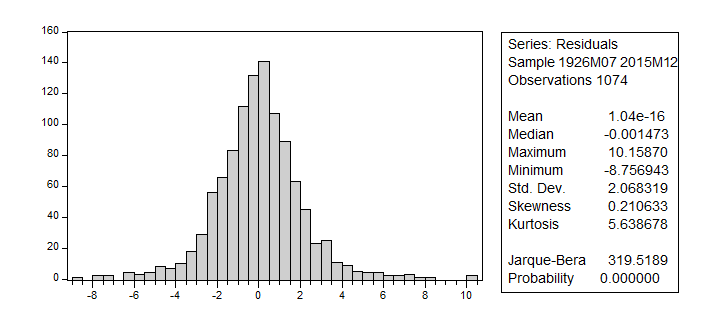
\includegraphics[]{hist.png}
%\caption{Add your caption here.}
%\label{fig:}
\end{figure}

Aquí también rechazamos la hipótesis nula que plantea el estadístico Jarque-Bera sobre la normalidad de los residuos; es decir, nuestro término de error no se distribuye siguiendo una Ley normal.

\section{Ejercicio 3} Contrasta mediante la prueba de Wald si el modelo con un factor es suficiente $H_0: \beta_3 = \beta_4 = 0$

\begin{table}[H]
\centering
\begin{tabular}{lrrr}
\multicolumn{1}{l}{Wald Test:}&\multicolumn{1}{c}{}&\multicolumn{1}{c}{}&\multicolumn{1}{c}{}\\
\multicolumn{2}{l}{Equation: EQ1}&\multicolumn{1}{c}{}&\multicolumn{1}{c}{}\\
[4.5pt] \hline \\ [-4.5pt]
\multicolumn{1}{l}{Test Statistic}&\multicolumn{1}{c}{Value}&\multicolumn{1}{c}{df}&\multicolumn{1}{c}{Probability}\\
[4.5pt] \hline \\ [-4.5pt]
\multicolumn{1}{l}{F-statistic}&\multicolumn{1}{c}{$151.9302$}&\multicolumn{1}{c}{(2, 1070)}&\multicolumn{1}{c}{$0.0000$}\\
\multicolumn{1}{l}{Chi-square}&\multicolumn{1}{c}{$303.8604$}&\multicolumn{1}{c}{$2$}&\multicolumn{1}{c}{$0.0000$}\\
[4.5pt] \hline \\ [-4.5pt]
\multicolumn{1}{c}{}&\multicolumn{1}{c}{}&\multicolumn{1}{c}{}&\multicolumn{1}{c}{}\\
\multicolumn{3}{l}{Null Hypothesis: C(3) = C(4) = 0}&\multicolumn{1}{c}{}\\
\multicolumn{2}{l}{Null Hypothesis Summary:}&\multicolumn{1}{c}{}&\multicolumn{1}{c}{}\\
[4.5pt] \hline \\ [-4.5pt]
\multicolumn{2}{l}{Normalized Restriction (= 0)}&\multicolumn{1}{c}{Value}&\multicolumn{1}{c}{Std. Err.}\\
[4.5pt] \hline \\ [-4.5pt]
\multicolumn{2}{l}{C(3)}&\multicolumn{1}{c}{$0.041632$}&\multicolumn{1}{c}{$0.020747$}\\
\multicolumn{2}{l}{C(4)}&\multicolumn{1}{c}{$-0.319994$}&\multicolumn{1}{c}{$0.018407$}\\
[4.5pt] \hline \\ [-4.5pt]
\multicolumn{3}{l}{Restrictions are linear in coefficients.}&\multicolumn{1}{c}{}\\
\end{tabular}
%\caption{Add your caption here.}
%\label{tab:}
\end{table}

Podemos \textbf{rechazar} la hipótesis nula acerca de que ambos coeficientes son 0, y por tanto podemos decir que el modelo con un solo factor no es suficiente para explicar nuestra variable dependiente (necesitamos, al menos, los tres factores).

\section{Ejercicio 4} Estamos interesados en analizar el posible efecto no lineal de \textit{smb} sobre el exceso de rendimiento de la cartera de Bienes de equipo y Comunicación \textit{(HiTec-Rf)}. Añade en el modelo la variable \textit{smb} al cuadrado e identifica el nuevo efecto marginal de \textit{smb} sobre el consumo. Contrasta si efectivamente este término cuadrático es necesario y explica las consecuencias que se derivan del resultado del contraste.

\begin{table}[H]
\centering
\begin{tabular}{lrrrr}
\multicolumn{3}{l}{Dependent Variable: HITEC-RF}&\multicolumn{1}{c}{}&\multicolumn{1}{c}{}\\
\multicolumn{2}{l}{Method: Least Squares}&\multicolumn{1}{c}{}&\multicolumn{1}{c}{}&\multicolumn{1}{c}{}\\
\multicolumn{2}{l}{Date: 09/02/20   Time: 15:17}&\multicolumn{1}{c}{}&\multicolumn{1}{c}{}&\multicolumn{1}{c}{}\\
\multicolumn{2}{l}{Sample: 1926M07 2015M12}&\multicolumn{1}{c}{}&\multicolumn{1}{c}{}&\multicolumn{1}{c}{}\\
\multicolumn{3}{l}{Included observations: 1074}&\multicolumn{1}{c}{}&\multicolumn{1}{c}{}\\
[4.5pt] \hline \\ [-4.5pt]
\multicolumn{1}{c}{Variable}&\multicolumn{1}{r}{Coefficient}&\multicolumn{1}{r}{Std. Error}&\multicolumn{1}{r}{t-Statistic}&\multicolumn{1}{r}{Prob.}\\
[4.5pt] \hline \\ [-4.5pt]
\multicolumn{1}{c}{C}&\multicolumn{1}{r}{$0.101179$}&\multicolumn{1}{r}{$0.064784$}&\multicolumn{1}{r}{$1.561796$}&\multicolumn{1}{r}{$0.1186$}\\
\multicolumn{1}{c}{RMRF}&\multicolumn{1}{r}{$0.986607$}&\multicolumn{1}{r}{$0.012609$}&\multicolumn{1}{r}{$78.24507$}&\multicolumn{1}{r}{$0.0000$}\\
\multicolumn{1}{c}{SMB}&\multicolumn{1}{r}{$0.012106$}&\multicolumn{1}{r}{$0.022784$}&\multicolumn{1}{r}{$0.531339$}&\multicolumn{1}{r}{$0.5953$}\\
\multicolumn{1}{c}{HML}&\multicolumn{1}{r}{$-0.330318$}&\multicolumn{1}{r}{$0.018639$}&\multicolumn{1}{r}{$-17.72158$}&\multicolumn{1}{r}{$0.0000$}\\
\multicolumn{1}{c}{SMB\textasciicircum 2}&\multicolumn{1}{r}{$0.004536$}&\multicolumn{1}{r}{$0.001474$}&\multicolumn{1}{r}{$3.077388$}&\multicolumn{1}{r}{$0.0021$}\\
[4.5pt] \hline \\ [-4.5pt]
\multicolumn{1}{l}{R-squared}&\multicolumn{1}{r}{$0.865536$}&\multicolumn{2}{l}{Mean dependent var}&\multicolumn{1}{r}{$0.663892$}\\
\multicolumn{1}{l}{Adjusted R-squared}&\multicolumn{1}{r}{$0.865033$}&\multicolumn{2}{l}{S.D. dependent var}&\multicolumn{1}{r}{$5.615646$}\\
\multicolumn{1}{l}{S.E. of regression}&\multicolumn{1}{r}{$2.063067$}&\multicolumn{2}{l}{Akaike info criterion}&\multicolumn{1}{r}{$4.290909$}\\
\multicolumn{1}{l}{Sum squared resid}&\multicolumn{1}{r}{$4549.927$}&\multicolumn{2}{l}{Schwarz criterion}&\multicolumn{1}{r}{$4.314090$}\\
\multicolumn{1}{l}{Log likelihood}&\multicolumn{1}{r}{$-2299.218$}&\multicolumn{2}{l}{Hannan-Quinn criter.}&\multicolumn{1}{r}{$4.299689$}\\
\multicolumn{1}{l}{F-statistic}&\multicolumn{1}{r}{$1720.274$}&\multicolumn{2}{l}{Durbin-Watson stat}&\multicolumn{1}{r}{$1.885307$}\\
\multicolumn{1}{l}{Prob(F-statistic)}&\multicolumn{1}{r}{$0.000000$}&\multicolumn{1}{c}{}&\multicolumn{1}{c}{}&\multicolumn{1}{c}{}\\
[4.5pt] \hline \\ [-4.5pt]
\end{tabular}
%\caption{Add your caption here.}
%\label{tab:}
\end{table}

Al añadir $smb^2$ podemos observar como la variable \textit{smb} pierde significatividad, lo que quiere decir que el efecto que aportaba ya viene recogido por la nueva variable, que sí es que es significativa. Además, todos los criterios de información (Akaike, Schwarz y Hannan-Quinn) disminuyen mientras que el $R^2$ aumenta, lo que nos indica que la estimación ha mejorado.

Si realizamos el test de Wald para $H_0: \beta_5 = 0$ veremos que debemos rechazar la hipótesis nula, confirmando lo que comentábamos en el apartado anterior.


\begin{table}[H]
\centering
\begin{tabular}{lrrr}
\multicolumn{1}{l}{Wald Test:}&\multicolumn{1}{c}{}&\multicolumn{1}{c}{}&\multicolumn{1}{c}{}\\
\multicolumn{2}{l}{Equation: EQ2}&\multicolumn{1}{c}{}&\multicolumn{1}{c}{}\\
[4.5pt] \hline \\ [-4.5pt]
\multicolumn{1}{l}{Test Statistic}&\multicolumn{1}{c}{Value}&\multicolumn{1}{c}{df}&\multicolumn{1}{c}{Probability}\\
[4.5pt] \hline \\ [-4.5pt]
\multicolumn{1}{l}{t-statistic}&\multicolumn{1}{c}{$3.077388$}&\multicolumn{1}{c}{$1069$}&\multicolumn{1}{c}{$0.0021$}\\
\multicolumn{1}{l}{F-statistic}&\multicolumn{1}{c}{$9.470314$}&\multicolumn{1}{c}{(1, 1069)}&\multicolumn{1}{c}{$0.0021$}\\
\multicolumn{1}{l}{Chi-square}&\multicolumn{1}{c}{$9.470314$}&\multicolumn{1}{c}{$1$}&\multicolumn{1}{c}{$0.0021$}\\
[4.5pt] \hline \\ [-4.5pt]
\multicolumn{1}{c}{}&\multicolumn{1}{c}{}&\multicolumn{1}{c}{}&\multicolumn{1}{c}{}\\
\multicolumn{2}{l}{Null Hypothesis: C(5) = 0}&\multicolumn{1}{c}{}&\multicolumn{1}{c}{}\\
\multicolumn{2}{l}{Null Hypothesis Summary:}&\multicolumn{1}{c}{}&\multicolumn{1}{c}{}\\
[4.5pt] \hline \\ [-4.5pt]
\multicolumn{2}{l}{Normalized Restriction (= 0)}&\multicolumn{1}{c}{Value}&\multicolumn{1}{c}{Std. Err.}\\
[4.5pt] \hline \\ [-4.5pt]
\multicolumn{2}{l}{C(5)}&\multicolumn{1}{c}{$0.004536$}&\multicolumn{1}{c}{$0.001474$}\\
[4.5pt] \hline \\ [-4.5pt]
\multicolumn{3}{l}{Restrictions are linear in coefficients.}&\multicolumn{1}{c}{}\\
\end{tabular}
%\caption{Add your caption here.}
%\label{tab:}
\end{table}


\section{Ejercicio 5} Partiendo del modelo inicial, se desea ahora analizar si la beta del exceso de rendimiento en el mercado $(\beta_2)$ ha cambiado tras la segunda guerra mundial. Crea una variable ficticia, que podemos denominar \textit{d1946}, que valga cero para los datos previos a 1946 (hasta 194512) y uno a partir de enero de 1946. Añade en el modelo la $d1946*(R_m-R_f)$. ¿Cuál es ahora el efecto marginal del exceso de rendimiento en el mercado sobre del exceso de rendimiento en la cartera HiTec? Contrasta si efectivamente este efecto es diferente antes y después de la segunda guerra mundial.

\begin{table}[H]
\centering
\begin{tabular}{lrrrr}
\multicolumn{3}{l}{Dependent Variable: HITEC-RF}&\multicolumn{1}{c}{}&\multicolumn{1}{c}{}\\
\multicolumn{2}{l}{Method: Least Squares}&\multicolumn{1}{c}{}&\multicolumn{1}{c}{}&\multicolumn{1}{c}{}\\
\multicolumn{2}{l}{Date: 09/02/20   Time: 15:17}&\multicolumn{1}{c}{}&\multicolumn{1}{c}{}&\multicolumn{1}{c}{}\\
\multicolumn{2}{l}{Sample: 1926M07 2015M12}&\multicolumn{1}{c}{}&\multicolumn{1}{c}{}&\multicolumn{1}{c}{}\\
\multicolumn{3}{l}{Included observations: 1074}&\multicolumn{1}{c}{}&\multicolumn{1}{c}{}\\
[4.5pt] \hline \\ [-4.5pt]
\multicolumn{1}{c}{Variable}&\multicolumn{1}{r}{Coefficient}&\multicolumn{1}{r}{Std. Error}&\multicolumn{1}{r}{t-Statistic}&\multicolumn{1}{r}{Prob.}\\
[4.5pt] \hline \\ [-4.5pt]
\multicolumn{1}{c}{C}&\multicolumn{1}{r}{$0.127978$}&\multicolumn{1}{r}{$0.064195$}&\multicolumn{1}{r}{$1.993583$}&\multicolumn{1}{r}{$0.0465$}\\
\multicolumn{1}{c}{RMRF}&\multicolumn{1}{r}{$0.963968$}&\multicolumn{1}{r}{$0.018982$}&\multicolumn{1}{r}{$50.78454$}&\multicolumn{1}{r}{$0.0000$}\\
\multicolumn{1}{c}{SMB}&\multicolumn{1}{r}{$0.041980$}&\multicolumn{1}{r}{$0.020734$}&\multicolumn{1}{r}{$2.024765$}&\multicolumn{1}{r}{$0.0431$}\\
\multicolumn{1}{c}{HML}&\multicolumn{1}{r}{$-0.305851$}&\multicolumn{1}{r}{$0.020473$}&\multicolumn{1}{r}{$-14.93923$}&\multicolumn{1}{r}{$0.0000$}\\
\multicolumn{1}{c}{D1946*RMRF}&\multicolumn{1}{r}{$0.040862$}&\multicolumn{1}{r}{$0.025967$}&\multicolumn{1}{r}{$1.573582$}&\multicolumn{1}{r}{$0.1159$}\\
[4.5pt] \hline \\ [-4.5pt]
\multicolumn{1}{l}{R-squared}&\multicolumn{1}{r}{$0.864659$}&\multicolumn{2}{l}{Mean dependent var}&\multicolumn{1}{r}{$0.663892$}\\
\multicolumn{1}{l}{Adjusted R-squared}&\multicolumn{1}{r}{$0.864152$}&\multicolumn{2}{l}{S.D. dependent var}&\multicolumn{1}{r}{$5.615646$}\\
\multicolumn{1}{l}{S.E. of regression}&\multicolumn{1}{r}{$2.069790$}&\multicolumn{2}{l}{Akaike info criterion}&\multicolumn{1}{r}{$4.297416$}\\
\multicolumn{1}{l}{Sum squared resid}&\multicolumn{1}{r}{$4579.627$}&\multicolumn{2}{l}{Schwarz criterion}&\multicolumn{1}{r}{$4.320596$}\\
\multicolumn{1}{l}{Log likelihood}&\multicolumn{1}{r}{$-2302.712$}&\multicolumn{2}{l}{Hannan-Quinn criter.}&\multicolumn{1}{r}{$4.306195$}\\
\multicolumn{1}{l}{F-statistic}&\multicolumn{1}{r}{$1707.385$}&\multicolumn{2}{l}{Durbin-Watson stat}&\multicolumn{1}{r}{$1.910821$}\\
\multicolumn{1}{l}{Prob(F-statistic)}&\multicolumn{1}{r}{$0.000000$}&\multicolumn{1}{c}{}&\multicolumn{1}{c}{}&\multicolumn{1}{c}{}\\
[4.5pt] \hline \\ [-4.5pt]
\end{tabular}
%\caption{Add your caption here.}
%\label{tab:}
\end{table}

El efecto que tiene ahora el exceso de rendimiento es menor respecto a nuestra ecuación principal \eqref{maineq}, debido a que parcialmente la nueva variable recoge los mismos datos, aunque esta no es significativa estadísticamente hablando.

\begin{table}[H]
\centering
\begin{tabular}{lrrr}
\multicolumn{1}{l}{Wald Test:}&\multicolumn{1}{c}{}&\multicolumn{1}{c}{}&\multicolumn{1}{c}{}\\
\multicolumn{2}{l}{Equation: EQ3}&\multicolumn{1}{c}{}&\multicolumn{1}{c}{}\\
[4.5pt] \hline \\ [-4.5pt]
\multicolumn{1}{l}{Test Statistic}&\multicolumn{1}{c}{Value}&\multicolumn{1}{c}{df}&\multicolumn{1}{c}{Probability}\\
[4.5pt] \hline \\ [-4.5pt]
\multicolumn{1}{l}{t-statistic}&\multicolumn{1}{c}{$-21.94391$}&\multicolumn{1}{c}{$1069$}&\multicolumn{1}{c}{$0.0000$}\\
\multicolumn{1}{l}{F-statistic}&\multicolumn{1}{c}{$481.5354$}&\multicolumn{1}{c}{(1, 1069)}&\multicolumn{1}{c}{$0.0000$}\\
\multicolumn{1}{l}{Chi-square}&\multicolumn{1}{c}{$481.5354$}&\multicolumn{1}{c}{$1$}&\multicolumn{1}{c}{$0.0000$}\\
[4.5pt] \hline \\ [-4.5pt]
\multicolumn{1}{c}{}&\multicolumn{1}{c}{}&\multicolumn{1}{c}{}&\multicolumn{1}{c}{}\\
\multicolumn{2}{l}{Null Hypothesis: C(5) = C(2)}&\multicolumn{1}{c}{}&\multicolumn{1}{c}{}\\
\multicolumn{2}{l}{Null Hypothesis Summary:}&\multicolumn{1}{c}{}&\multicolumn{1}{c}{}\\
[4.5pt] \hline \\ [-4.5pt]
\multicolumn{2}{l}{Normalized Restriction (= 0)}&\multicolumn{1}{c}{Value}&\multicolumn{1}{c}{Std. Err.}\\
[4.5pt] \hline \\ [-4.5pt]
\multicolumn{2}{l}{-C(2) + C(5)}&\multicolumn{1}{c}{$-0.923106$}&\multicolumn{1}{c}{$0.042067$}\\
[4.5pt] \hline \\ [-4.5pt]
\multicolumn{3}{l}{Restrictions are linear in coefficients.}&\multicolumn{1}{c}{}\\
\end{tabular}
%\caption{Add your caption here.}
%\label{tab:}
\end{table}

Realizando el contraste para comprobar si el efecto es diferente antes y después de la segunda guerra mundial ($H_0: \beta_2 = \beta_5$), debemos rechazar la hipótesis nula, por lo que podemos determinar que los efectos son diferentes antes y después de la segunda guerra mundial.

\section{Ejercicio 6} Estima de nuevo el modelo básico de tres factores solicitando una estimación robusta de la matriz de varianzas de los parámetros. Compara los resultados de esta estimación con la obtenida en el primer punto. Puedes probar diferentes fórmulas para la estimación de la matriz de varianzas para ver si los resultados varían.

\begin{table}[H]
\centering
\begin{tabular}{lrrrr}
\multicolumn{3}{l}{Dependent Variable: HITEC-RF}&\multicolumn{1}{c}{}&\multicolumn{1}{c}{}\\
\multicolumn{2}{l}{Method: Least Squares}&\multicolumn{1}{c}{}&\multicolumn{1}{c}{}&\multicolumn{1}{c}{}\\
\multicolumn{2}{l}{Date: 09/02/20   Time: 15:17}&\multicolumn{1}{c}{}&\multicolumn{1}{c}{}&\multicolumn{1}{c}{}\\
\multicolumn{2}{l}{Sample: 1926M07 2015M12}&\multicolumn{1}{c}{}&\multicolumn{1}{c}{}&\multicolumn{1}{c}{}\\
\multicolumn{3}{l}{Included observations: 1074}&\multicolumn{1}{c}{}&\multicolumn{1}{c}{}\\
\multicolumn{5}{l}{White-Hinkley (HC1) heteroskedasticity consistent standard errors and}\\
\multicolumn{2}{l}{covariance}&\multicolumn{1}{c}{}&\multicolumn{1}{c}{}&\multicolumn{1}{c}{}\\
[4.5pt] \hline \\ [-4.5pt]
\multicolumn{1}{c}{Variable}&\multicolumn{1}{r}{Coefficient}&\multicolumn{1}{r}{Std. Error}&\multicolumn{1}{r}{t-Statistic}&\multicolumn{1}{r}{Prob.}\\
[4.5pt] \hline \\ [-4.5pt]
\multicolumn{1}{c}{C}&\multicolumn{1}{r}{$0.138453$}&\multicolumn{1}{r}{$0.062816$}&\multicolumn{1}{r}{$2.204108$}&\multicolumn{1}{r}{$0.0277$}\\
\multicolumn{1}{c}{RMRF}&\multicolumn{1}{r}{$0.986237$}&\multicolumn{1}{r}{$0.019642$}&\multicolumn{1}{r}{$50.21179$}&\multicolumn{1}{r}{$0.0000$}\\
\multicolumn{1}{c}{SMB}&\multicolumn{1}{r}{$0.041632$}&\multicolumn{1}{r}{$0.027664$}&\multicolumn{1}{r}{$1.504943$}&\multicolumn{1}{r}{$0.1326$}\\
\multicolumn{1}{c}{HML}&\multicolumn{1}{r}{$-0.319994$}&\multicolumn{1}{r}{$0.032304$}&\multicolumn{1}{r}{$-9.905557$}&\multicolumn{1}{r}{$0.0000$}\\
[4.5pt] \hline \\ [-4.5pt]
\multicolumn{1}{l}{R-squared}&\multicolumn{1}{r}{$0.864345$}&\multicolumn{2}{l}{Mean dependent var}&\multicolumn{1}{r}{$0.663892$}\\
\multicolumn{1}{l}{Adjusted R-squared}&\multicolumn{1}{r}{$0.863965$}&\multicolumn{2}{l}{S.D. dependent var}&\multicolumn{1}{r}{$5.615646$}\\
\multicolumn{1}{l}{S.E. of regression}&\multicolumn{1}{r}{$2.071217$}&\multicolumn{2}{l}{Akaike info criterion}&\multicolumn{1}{r}{$4.297867$}\\
\multicolumn{1}{l}{Sum squared resid}&\multicolumn{1}{r}{$4590.235$}&\multicolumn{2}{l}{Schwarz criterion}&\multicolumn{1}{r}{$4.316411$}\\
\multicolumn{1}{l}{Log likelihood}&\multicolumn{1}{r}{$-2303.955$}&\multicolumn{2}{l}{Hannan-Quinn criter.}&\multicolumn{1}{r}{$4.304891$}\\
\multicolumn{1}{l}{F-statistic}&\multicolumn{1}{r}{$2272.552$}&\multicolumn{2}{l}{Durbin-Watson stat}&\multicolumn{1}{r}{$1.911409$}\\
\multicolumn{1}{l}{Prob(F-statistic)}&\multicolumn{1}{r}{$0.000000$}&\multicolumn{2}{l}{Wald F-statistic}&\multicolumn{1}{r}{$914.4917$}\\
\multicolumn{1}{l}{Prob(Wald F-statistic)}&\multicolumn{1}{r}{$0.000000$}&\multicolumn{1}{c}{}&\multicolumn{1}{c}{}&\multicolumn{1}{c}{}\\
[4.5pt] \hline \\ [-4.5pt]
\end{tabular}
%\caption{Add your caption here.}
%\label{tab:}
\end{table}


\begin{table}[H]
\centering
\begin{tabular}{lrrrr}
\multicolumn{3}{l}{Dependent Variable: HITEC-RF}&\multicolumn{1}{c}{}&\multicolumn{1}{c}{}\\
\multicolumn{2}{l}{Method: Least Squares}&\multicolumn{1}{c}{}&\multicolumn{1}{c}{}&\multicolumn{1}{c}{}\\
\multicolumn{2}{l}{Date: 09/02/20   Time: 15:17}&\multicolumn{1}{c}{}&\multicolumn{1}{c}{}&\multicolumn{1}{c}{}\\
\multicolumn{2}{l}{Sample: 1926M07 2015M12}&\multicolumn{1}{c}{}&\multicolumn{1}{c}{}&\multicolumn{1}{c}{}\\
\multicolumn{3}{l}{Included observations: 1074}&\multicolumn{1}{c}{}&\multicolumn{1}{c}{}\\
\multicolumn{5}{l}{MacKinnon-White (HC2) heteroskedasticity-consistent standard errors \&}\\
\multicolumn{2}{l}{covariance}&\multicolumn{1}{c}{}&\multicolumn{1}{c}{}&\multicolumn{1}{c}{}\\
[4.5pt] \hline \\ [-4.5pt]
\multicolumn{1}{c}{Variable}&\multicolumn{1}{r}{Coefficient}&\multicolumn{1}{r}{Std. Error}&\multicolumn{1}{r}{t-Statistic}&\multicolumn{1}{r}{Prob.}\\
[4.5pt] \hline \\ [-4.5pt]
\multicolumn{1}{c}{C}&\multicolumn{1}{r}{$0.138453$}&\multicolumn{1}{r}{$0.062892$}&\multicolumn{1}{r}{$2.201430$}&\multicolumn{1}{r}{$0.0279$}\\
\multicolumn{1}{c}{RMRF}&\multicolumn{1}{r}{$0.986237$}&\multicolumn{1}{r}{$0.019916$}&\multicolumn{1}{r}{$49.51928$}&\multicolumn{1}{r}{$0.0000$}\\
\multicolumn{1}{c}{SMB}&\multicolumn{1}{r}{$0.041632$}&\multicolumn{1}{r}{$0.028066$}&\multicolumn{1}{r}{$1.483382$}&\multicolumn{1}{r}{$0.1383$}\\
\multicolumn{1}{c}{HML}&\multicolumn{1}{r}{$-0.319994$}&\multicolumn{1}{r}{$0.032995$}&\multicolumn{1}{r}{$-9.698145$}&\multicolumn{1}{r}{$0.0000$}\\
[4.5pt] \hline \\ [-4.5pt]
\multicolumn{1}{l}{R-squared}&\multicolumn{1}{r}{$0.864345$}&\multicolumn{2}{l}{Mean dependent var}&\multicolumn{1}{r}{$0.663892$}\\
\multicolumn{1}{l}{Adjusted R-squared}&\multicolumn{1}{r}{$0.863965$}&\multicolumn{2}{l}{S.D. dependent var}&\multicolumn{1}{r}{$5.615646$}\\
\multicolumn{1}{l}{S.E. of regression}&\multicolumn{1}{r}{$2.071217$}&\multicolumn{2}{l}{Akaike info criterion}&\multicolumn{1}{r}{$4.297867$}\\
\multicolumn{1}{l}{Sum squared resid}&\multicolumn{1}{r}{$4590.235$}&\multicolumn{2}{l}{Schwarz criterion}&\multicolumn{1}{r}{$4.316411$}\\
\multicolumn{1}{l}{Log likelihood}&\multicolumn{1}{r}{$-2303.955$}&\multicolumn{2}{l}{Hannan-Quinn criter.}&\multicolumn{1}{r}{$4.304891$}\\
\multicolumn{1}{l}{F-statistic}&\multicolumn{1}{r}{$2272.552$}&\multicolumn{2}{l}{Durbin-Watson stat}&\multicolumn{1}{r}{$1.911409$}\\
\multicolumn{1}{l}{Prob(F-statistic)}&\multicolumn{1}{r}{$0.000000$}&\multicolumn{2}{l}{Wald F-statistic}&\multicolumn{1}{r}{$888.5525$}\\
\multicolumn{1}{l}{Prob(Wald F-statistic)}&\multicolumn{1}{r}{$0.000000$}&\multicolumn{1}{c}{}&\multicolumn{1}{c}{}&\multicolumn{1}{c}{}\\
[4.5pt] \hline \\ [-4.5pt]
\end{tabular}
%\caption{Add your caption here.}
%\label{tab:}
\end{table}

Aquí hemos empleado el método de MCO pero estimando la matriz de varianzas-covarianzas para que sea consistente (robusta) mediante dos métodos distintos: el primero es usando White y el segundo HC\footnote{No usamos HAC porque ya hemos comprobado que los residuos no están autocorrelados.} (heterokedasticity consistent). 

Podemos observar que los coeficientes no cambian, ya que el estimador sigue siendo insesgado; sólo hemos cambiado la forma de calcular la matriz de varianzas-covarianzas, y la única diferencia es que el error típico de nuestros estimadores es distinto.

\section{Código}

A continuación dejo el código empleado para replicar los resultados obtenidos mediante un programa de Eviews, así como mi repositorio en \href{https://github.com/mdelallave/Econometria_financiera/tree/master/primera_entrega}{GitHub} donde también se puede ver el código empleado en \LaTeX.\footnote{Colocar el fichero de datos en la misma carpeta que el programa de Eviews.}

\verbatiminput{codigo.tex}

\end{document}
